The showcase uses the architecture as a base and adds features referencing the research topic. The simulation image of the architecture is used as a base for the one in the showcase. Three more images are added for containers that run a \acs{slam} algorithm, a path planning algorithm, and a \acs{qrcode} detector. These algorithms and the detector are clarified in the chapter of the research topic.

\begin{figure}[!h]
  \centering
  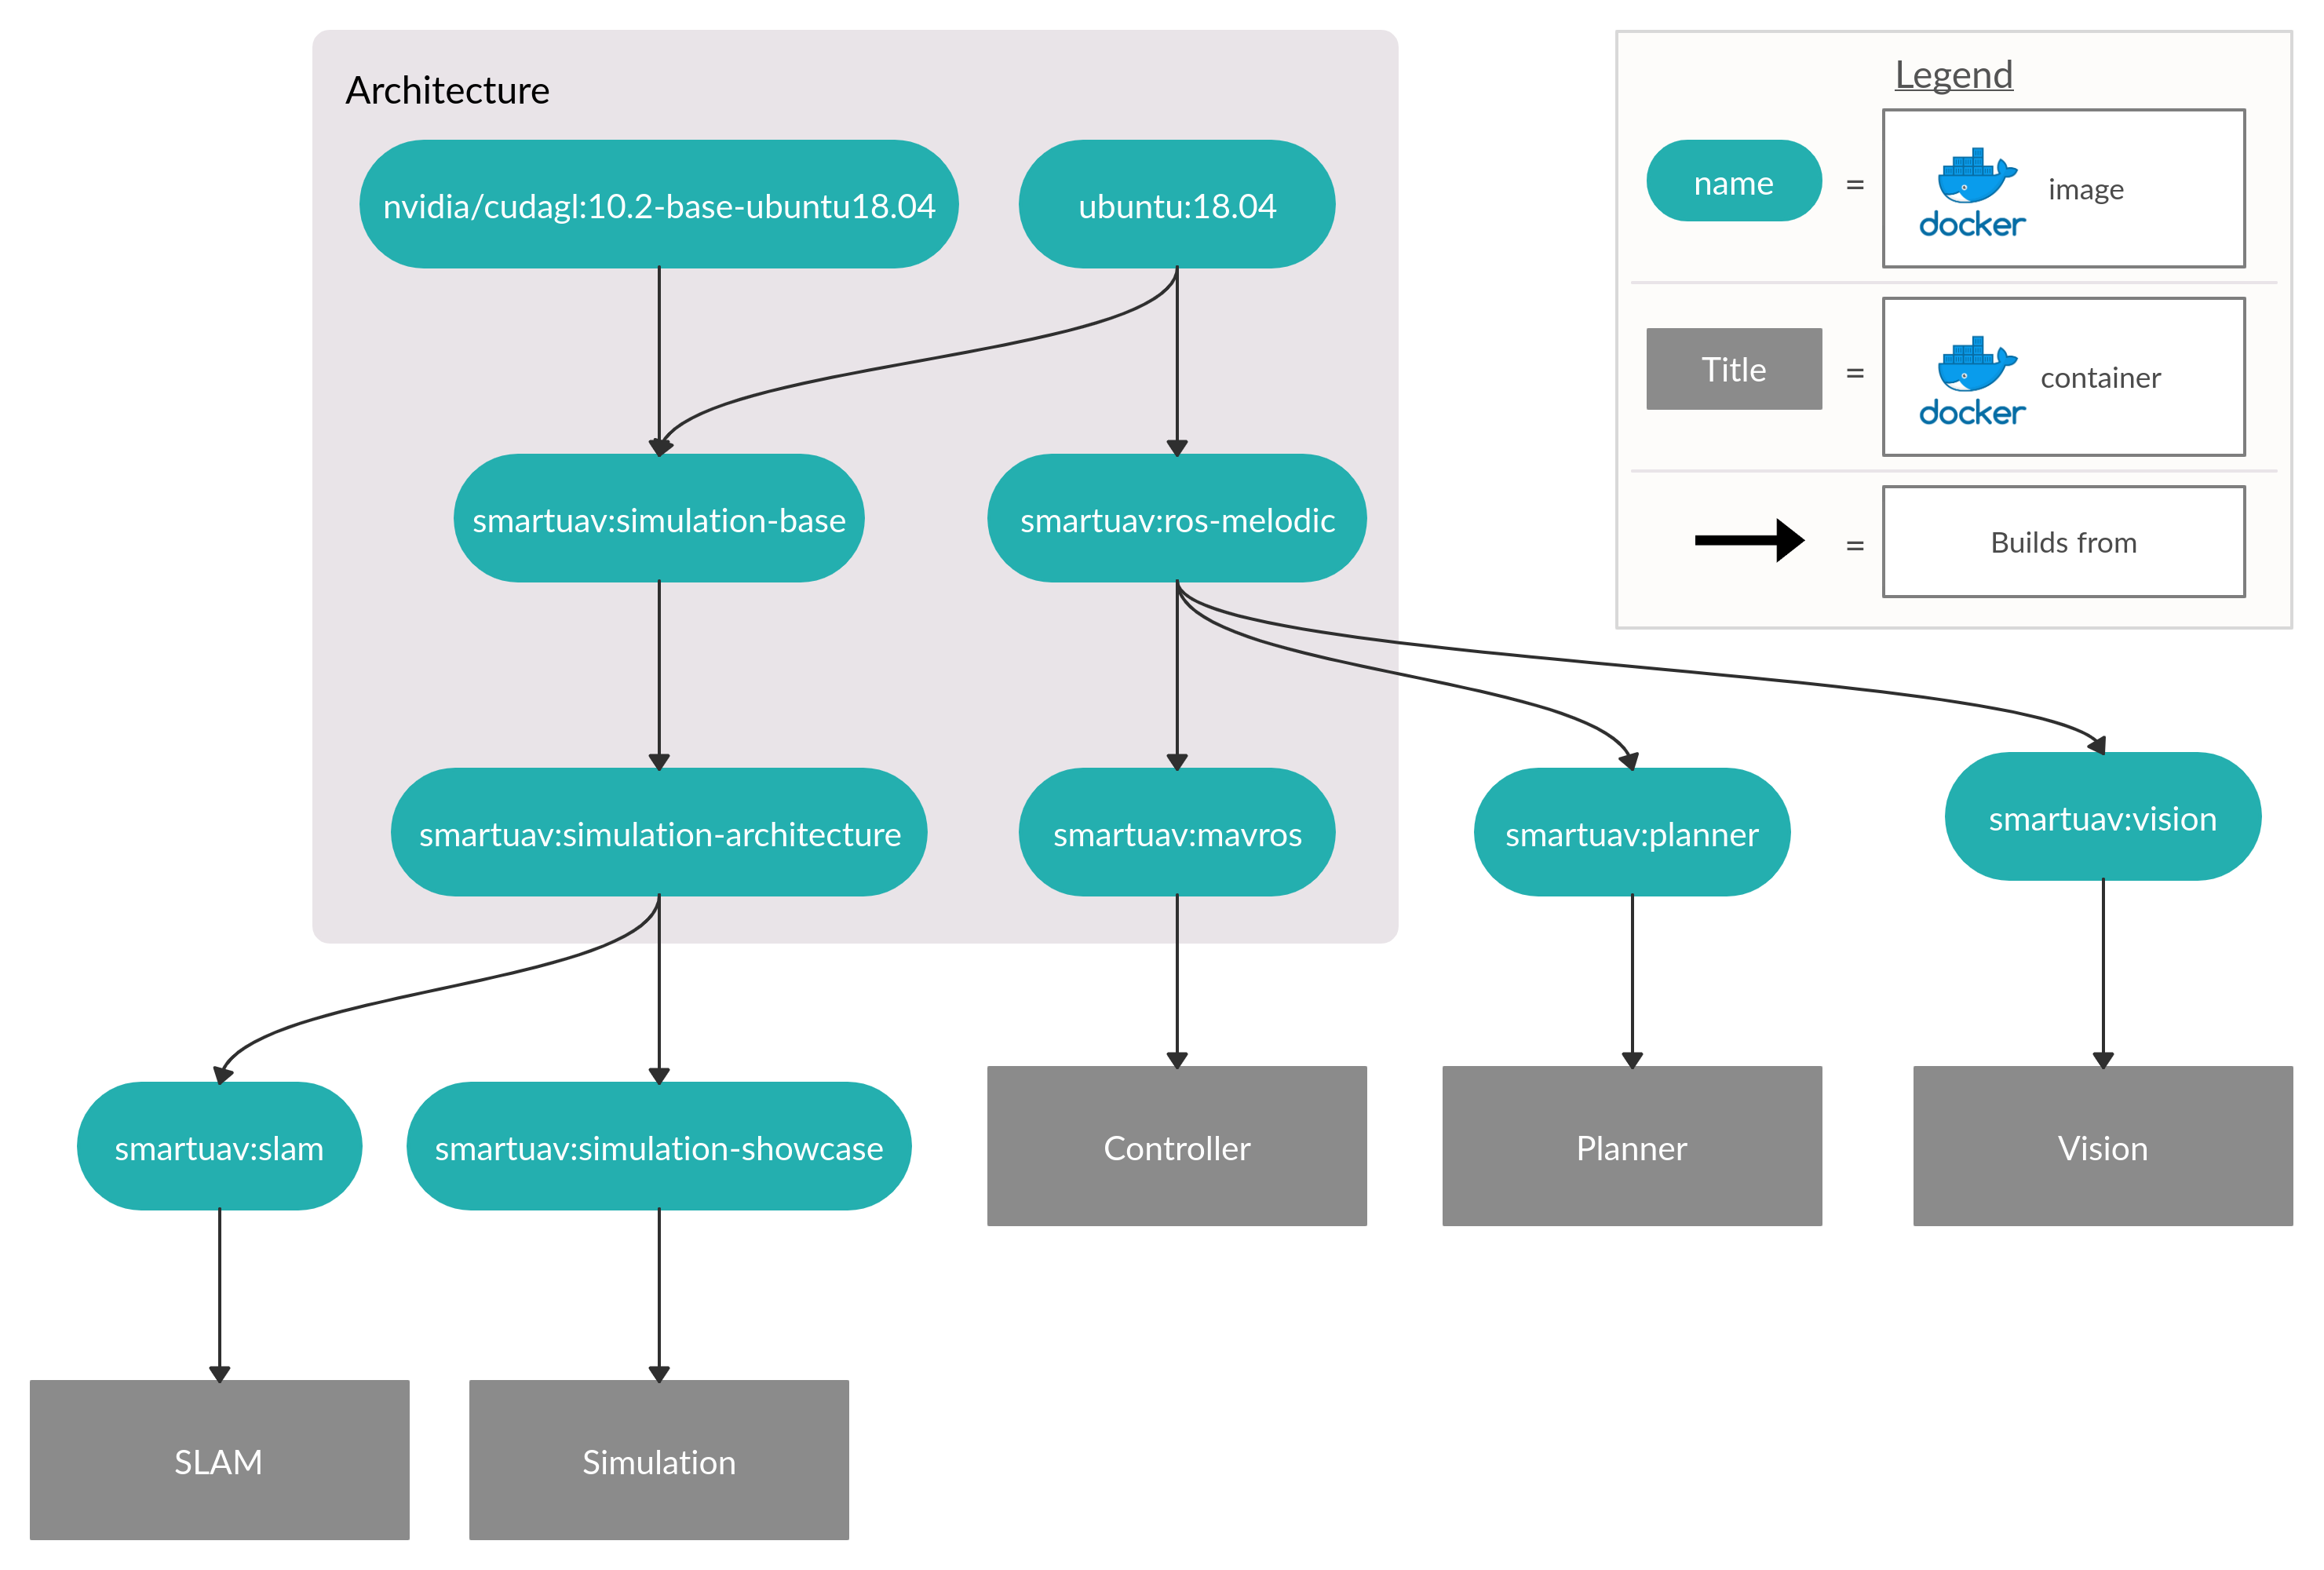
\includegraphics[width=\linewidth]{images/showcase_images.png}
  \caption{Docker images showcase}
\end{figure}

\clearpage

The showcase is used to conduct research, visualize this research, and show the capabilities of the architecture. Figure~\ref{fig:showcase_containers} visualizes which containers are run in the showcase and how there are connected.

\begin{figure}[!h]
  \centering
  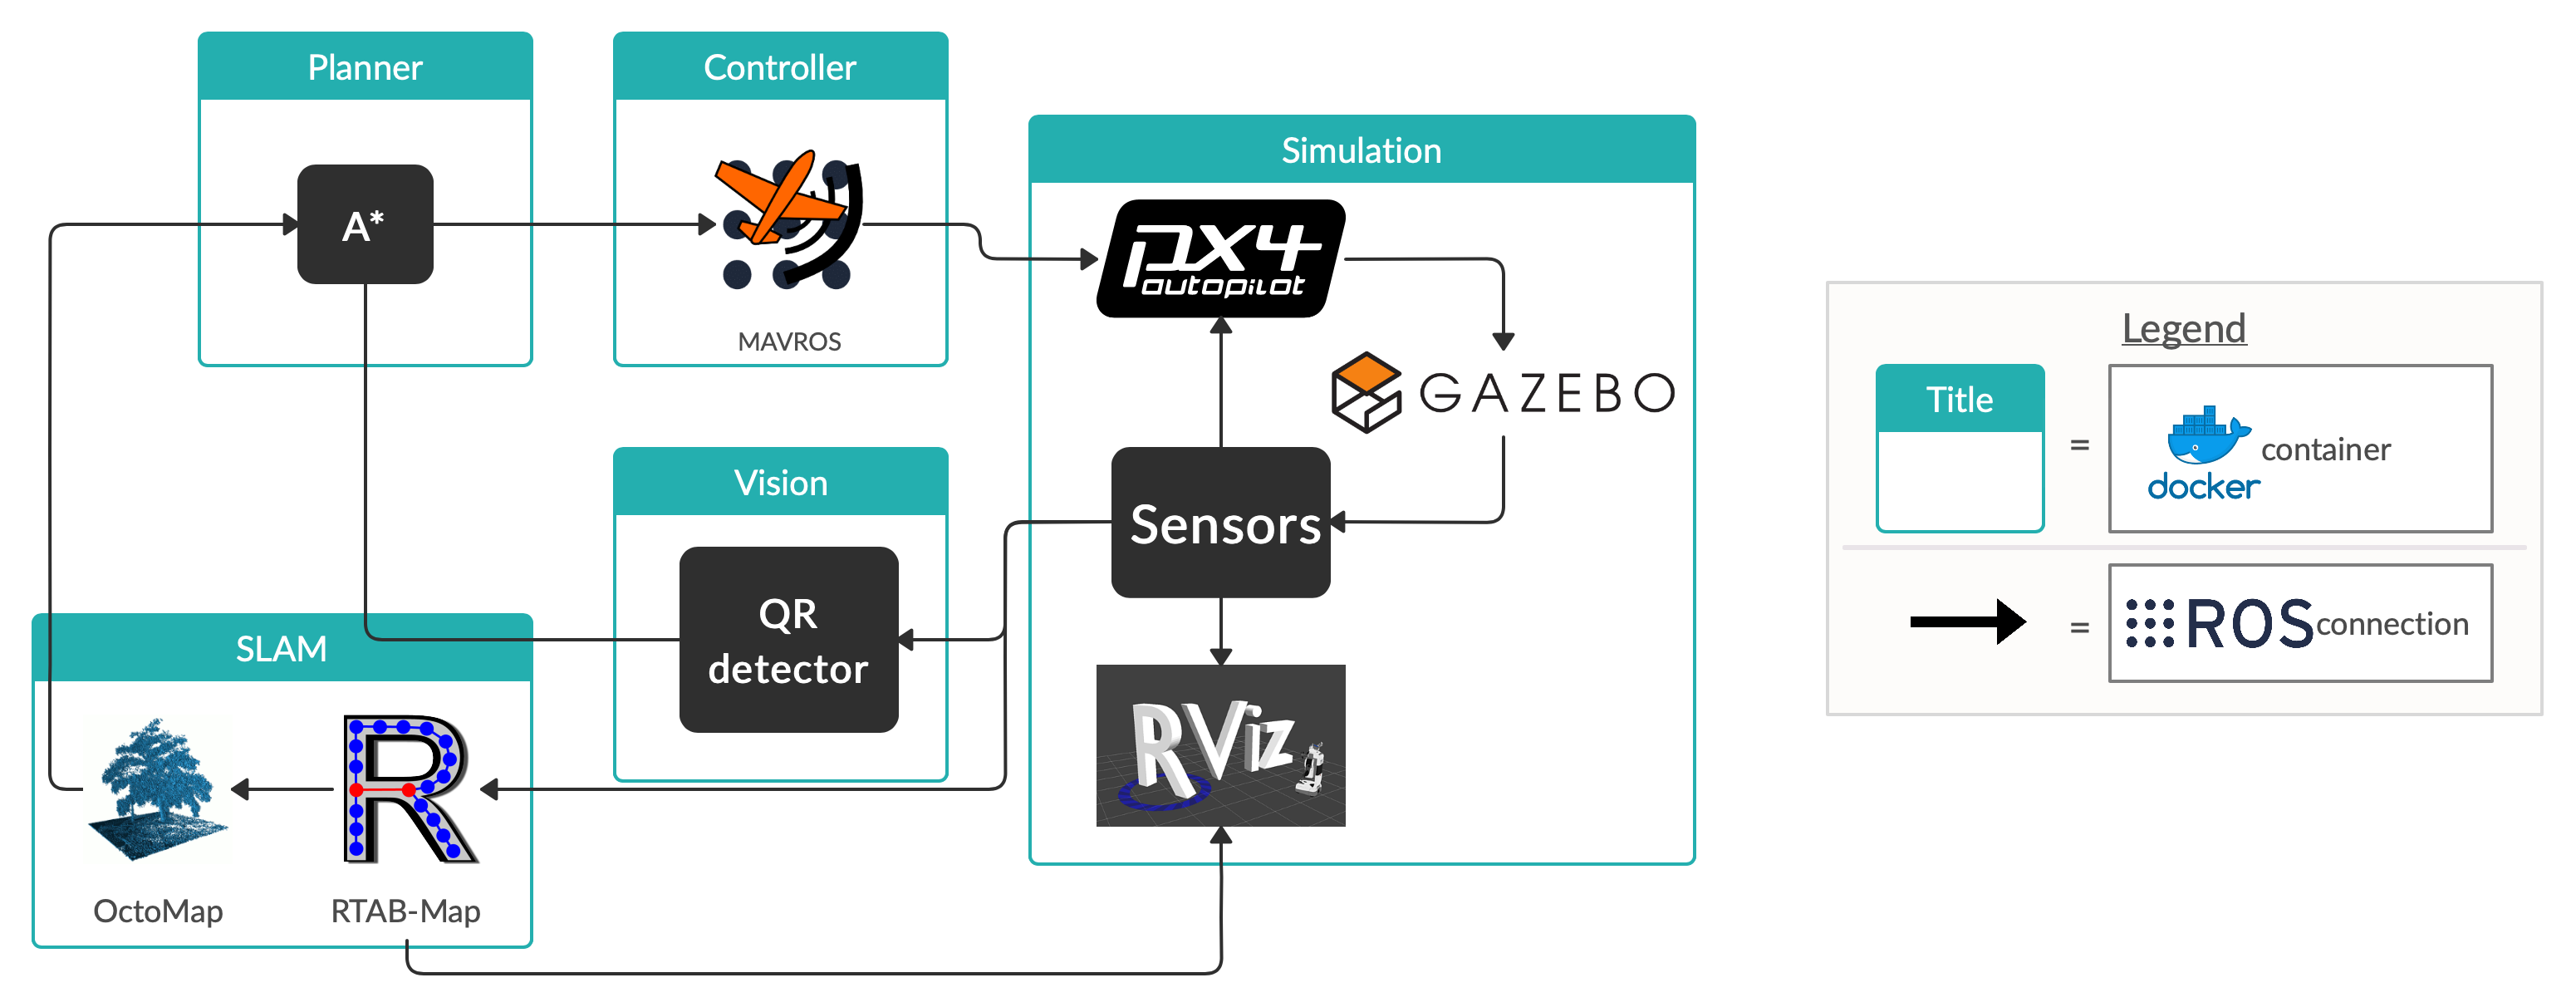
\includegraphics[width=\linewidth]{images/showcase_containers.png}
  \caption{Docker containers showcase}
  \label{fig:showcase_containers}
\end{figure}